\chapter{Physikalische Grundlagen}
In disem Kapitel wird der physikalische Hintergrund zu dieser Arbeit behandelt.
Zuerst wird auf den Aufbau des IceCube-Neutrino-Observatoriums eingegangen und dabei die Funktionsweise des Detektors erläutert.
Anschließend werden kurz wichtige Aspekte der Neutrinophysik aufgeführt.

% ICECUBE
\section{IceCube-Neutrino-Observatorium} \label{sec:icecube}

IceCube ist ein Hochenergie-Neutrino-Observatorium am geographischen Südpol.
Der Detektor befindet sich in einer Tiefe von \SIrange{1450}{2450}{\metre} im antarktischen Eis und deckt ein Volumen von \SI{1}{\kilo\metre^3} ab.\cite{icecube_detector}
An 86 Strings sind in regelmäßigen Abständen DOMs (Digital Optical Module) angebracht.
Der Detektoraufbau ist schematisch in der \autoref{fig:detector} dargestellt.
\begin{figure}
    \centering
    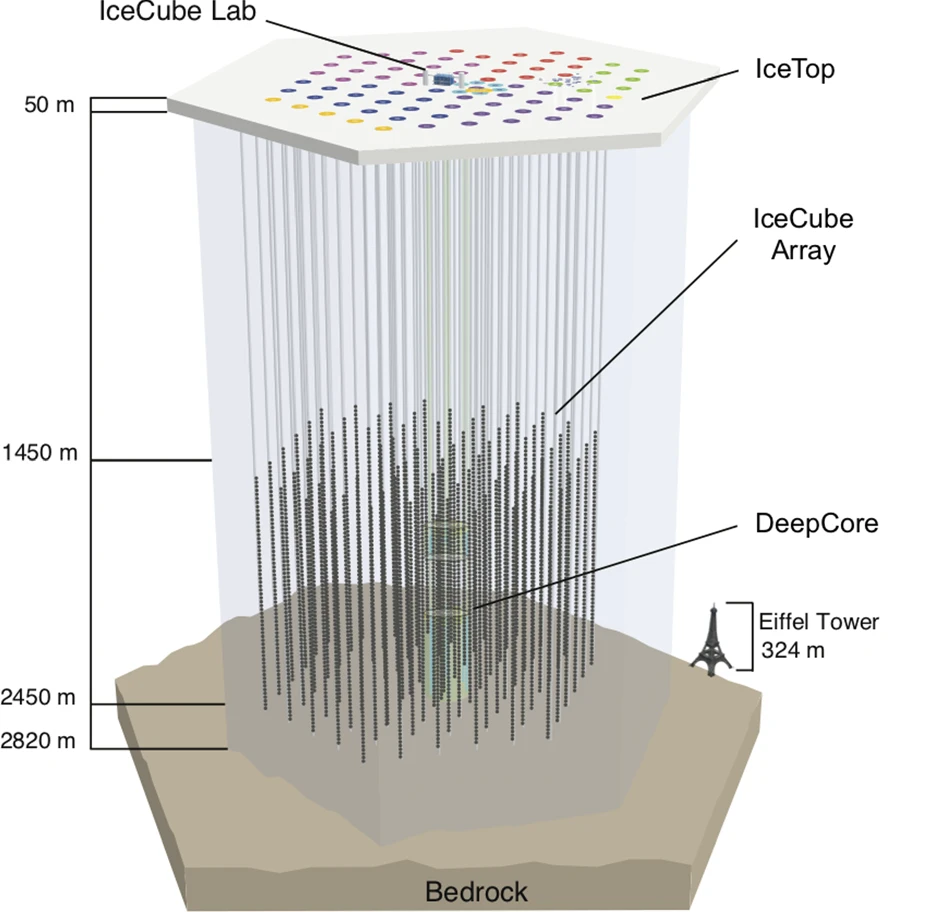
\includegraphics[width=0.5\textwidth]{Plots/detector2.png}
    \caption[IceCube-Detektor und IceTop Array]{Schematische Darstellung des sich im antarktischen Eis befindenden IceCube-Detektors und des IceTop Arrays.
    IceCube liegt \SIrange{1450}{2450}{\metre} unter dem Eis und beinhaltet den Teildetektor DeepCore.
    Jeder Punkt stellt einen DOM und jeder Kreis eine IceTop-Station auf der Eisoberfläche dar \cite{Ahlers_2018}.
    }
    \label{fig:detector}
\end{figure}

Ein großer Teil des DOMs besteht aus einem Photomultiplier der Licht im Wellenlängenbereich \SIrange{300}{650}{\nano\metre} registriert.
Hochenergetische Neutrinos wechselwirken mit dem Eis und zerfallen in Leptonen (Elektron, Myon, Tau-Lepton).
Aufgrund der Enegieerhaltung besitzen die Leptonen eine hohe kinetische Energie.
Sie bewegen sich mit einer Geschwindigkeit $v$ die größer als die Lichtgeschwindigkeit im Medium $c_m$ ist durch das Eis.
Dabei wird kegelförmig Cherenkov-Strahlung\cite{landau2013electrodynamics} im Winkel $\theta$ zur Teilchenbahn nach
\begin{equation*}
\cos(\theta) = \frac{c_m}{v}
\end{equation*}
emittiert.
Treffen die Photonen auf die Photomultiplier wird eine Ladung erzeugt, diese wird verstärkt und digitalisiert.
Das Signal wird von den DOMs an die nahliegende Amundsen-Scott Südpolstation übertragen.
\\
Die durch das Licht erzeugte Signatur im Detektor, gibt Kenntniss über die Energie und Herkunft des Neutrinos.
IceCube ist darauf ausgelegt Neutrinos mit Energien im \si{\tera\eV}-Bereich\cite{Ahlers_2018} zu detektieren.

% NEUTRINO
\section{Neutrino-Astronomie}
Neutrinos sind aufgrund ihrer Eigenschaften optimale Botenteilchen.
Sie sind neutral geladen und wechselwirken daher nicht mit elektromagnetischen Feldern.
Aufgrund der sehr geringen Masse sind auch gravitative Effekte nicht von Bedeutung.
\\
Die geringe Wechselwirkungswahrscheinlichkeit der Neutrinos hat den Vorteil, dass diese unabgelenkt von weitentfernten kosmischen Quellen auf der Erde ankommen.
Sie tragen Informationen der ursprünglichen Quelle in sich.
Zum einen lässt die Neutrinoenergie Rückschlüsse auf die Art der Quelle zu.
Zum anderen kann über die Rekonstruktion der Neutrinobahn die Quelle lokalisiert werden.
\\
Aus dem gleichen Grund gestaltet sich die Detektion der Neutrinos als große Herausforderung.
Um Neutrinos zu detektieren werden große Detektorvolumen benötigt.
IceCube deckt den Hochenergiebereich ab, wobei bis heute auch die höchsten Energien ($\gtrsim$ \SI{100}{\peta\eV}) verborgen bleiben.

\begin{figure}
    \centering
    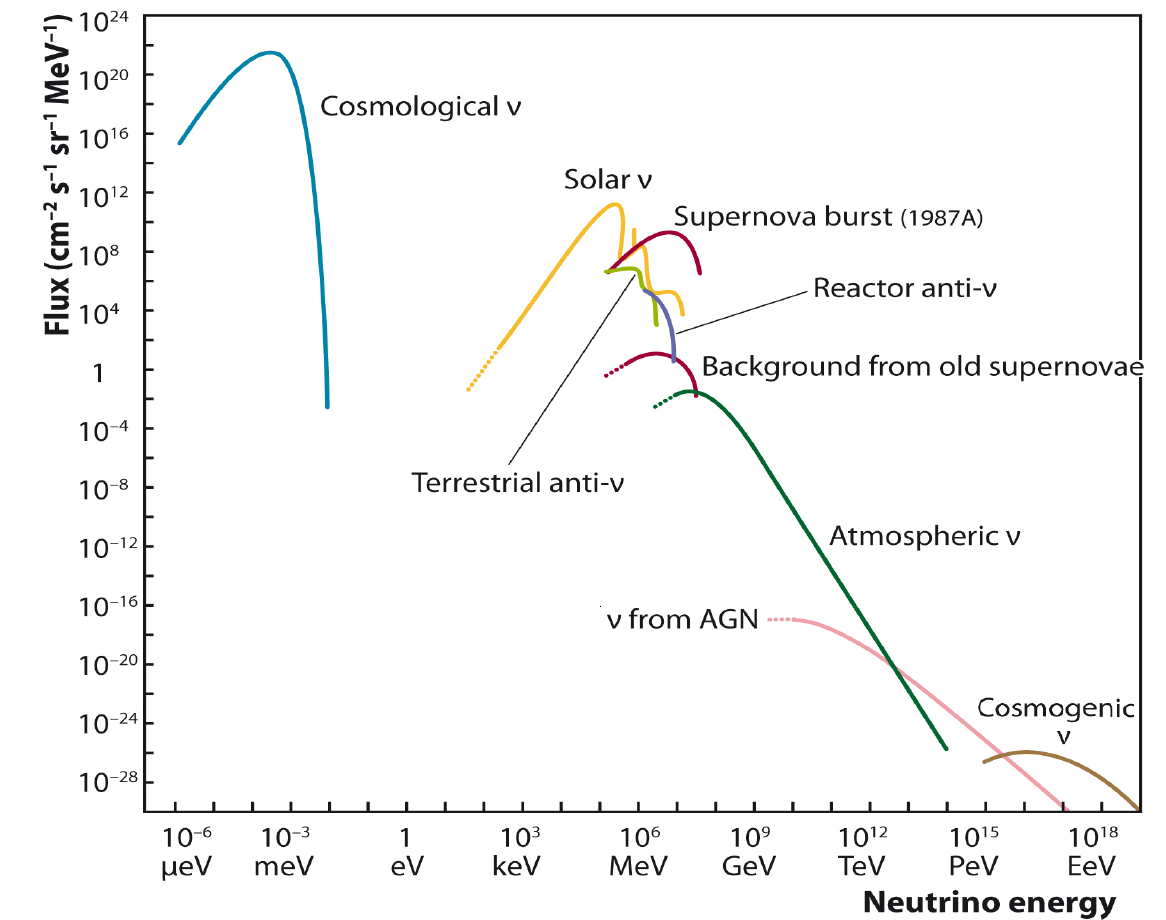
\includegraphics[width=0.7\textwidth]{Plots/neutrinoflux.png}
    \caption[Neutrinofluss in Abhängigkeit der Energie]{Neutrinofluss in Abhängigkeit der Energie für verschiedene Neutrinoquellen \cite{Spiering_2012}.
    }
    \label{fig:neutrino_flux}
\end{figure}

Der Neutrinofluss der energiereichsten Neutrinos ist so gering, dass zum Nachweis ein Detektor notwendig ist, der 1 bis 3 Größenordnungen größer als IceCube ist.
Wie in \autoref{fig:neutrino_flux} zu erkennen ist, handelt es sich bei den in IceCube detektierten Neutrinos um atmosphärische Neutrinos und Neutrinos aus aktiven Galaxiekernen (AGN).
\\
Atmosphärische Neutrinos entstehen bei der Kollision hochenergetischer Teilchen mit der Erdatmosphäre.
Kosmische Strahlung besteht überwiegend aus geladenen Kernen.
Diese wechselwirken mit den Atomkernen in der Atmosphäre und zerfallen über die schwache Wechselwirkung.
Es wird ein Neutrino frei.
\\
Ein Ziel von IceCube ist die Gewinnung neuer Erkenntnisse über die Quellen kosmischer Strahlung, in denen auch hochenergetische Neutrinos erzeugt werden.
\\
Es existieren drei Generationen (Flavor) von Neutrinos, das Elektron-Neutrino $\nu_e$, das Myon-Neutrino $\nu_\mu$ und das Tau-Neutrino $\nu_\tau$.
Aus Modellen, die verschiedene Neutrinoquellen betrachten geht hervor, dass Neutrinos im Verhältnis $\nu_e$:$\nu_\mu$:$\nu_\tau$ = $1$:$2$:$0$ entstehen.
Auf der Erde werden alle Neutrinos gleichermaße gemessen: $\nu_e$:$\nu_\mu$:$\nu_\tau$ = $1$:$1$:$1$.
Grund sind die Neutrino-Oszillationen\cite{oscillation_bilenky,oscillation_wolfenstein}, die einen Wechsel zwischen Generationen ohne weitere Wechselwirkung erlauben.
\\
Die drei Neutrinoarten erzeugen im Detektor unterschiedliche Signaturen und ermöglichen eine Bestimmung des Flavors.
Eine \textbf{Kaskade}\cite{signature_e} wird beobachtet, wenn bei der Wechselwirkung eines $\nu_e$ ein $e^{\pm}$ ensteht.
Aufgrund von Bremsstrahlungs- und Paarproduktionsprozessen nimmt die Energie ab.
Am Ort der Wechselwirkung befindet sich das Energiemaximum.
\\
Reagiert ein $\nu_\mu$ mit dem Eis, so entsteht als sekundäres Teilchen ein Myon $\mu$.
Dieses propagiert durch das Eis und verliert Energie in Form von Ionisation, Paarerzeugung, Bremsstrahlung und photonuklearen Wechselwirkungen.
Die Signatur entspricht einer \textbf{Spur} mit abnehmender Energie.
\\
Der \textbf{Double Bang} ("`Doppel-Knall"') wird durch ein $\nu_\tau$ hervorgerufen.
Bei der Wechselwirkung entsteht ein Tauon $\tau$ und es wird eine Kaskade erzeugt.
Der Zerfall des Tauons, nach der mittleren Lebensdauer von $\SI{290.3(5)e-15}{\second}$ \cite{pdg} führt zu einer weiteren Kaskade.
So ein Ereignis wäre ein klarer Nachweis für ein $\nu_\tau$.